%% В этот файл не предполагается вносить изменения

% В этом файле следует указать информацию о себе
% и выполняемой работе.

\documentclass [fontsize=14pt, paper=a4, pagesize, DIV=calc]%
{scrartcl}
% ВНИМАНИЕ! Для использования глав поменять
% scrartcl на scrreprt

% Здесь ничего не менять
\usepackage [T2A] {fontenc}   % Кириллица в PDF файле
\usepackage [utf8] {inputenc} % Кодировка текста: utf-8
\usepackage [russian] {babel} % Переносы, лигатуры

%%%%%%%%%%%%%%%%%%%%%%%%%%%%%%%%%%%%%%%%%%%%%%%%%%%%%%%%%%%%%%%%%%%%%%%%
% Создание макроса управления элементами, специфичными
% для вида работы (курс., бак., маг.)
% Здесь ничего не менять:
\usepackage{ifthen}
\newcounter{worktype}
\newcommand{\typeOfWork}[1]
{
	\setcounter{worktype}{#1}
}

% ВНИМАНИЕ!
% Укажите тип работы: 0 - курсовая, 1 - бак., 2 - маг.,
% 3 - бакалаврская с главами.
\typeOfWork{1}
% Считается, что курсовая и бак. бьются на разделы (section) и
% подразделы (subsection), а маг. — на главы (chapter), разделы и
%  подразделы. Если хочется,
% чтобы бак. была с главами (например, если она большая),
% надо выбрать опцию 3.

% Если при выборе 2 или 3 вы забудете поменять класс
% документа на scrreprt (см. выше, в самом начале),
% то получите ошибку:
% ./aux/appearance.tex:52: Package scrbase Error: unknown option ` chapterprefix=

%%%%%%%%%%%%%%%%%%%%%%%%%%%%%%%%%%%%%%%%%%%%%%%%%%%%%%%%%%%%%%%%%%%%%%%%
% Информация об авторе и работе для титульной страницы

\usepackage {titling}

% Имя автора в именительном падеже (для маг.)
\newcommand {\me}{%
И.\,И.~Иванов%
}

% Имя автора в родительном падеже (для курсовой и бак.)
\newcommand {\byme}{%
В.\,М.~Ложкиной%
}

% Научный руководитель
\newcommand{\supervisor}%
{старший преподаватель кафедры информатики и вычислительного эксперимента В.\,Н.~Брагилевский}

% идентифицируем пол (только для курсовой и бак.)
\newcommand{\bystudent}{
Студентки % Для курсовой: с большой буквы
}

% Год публикации
\date{2018}

% Название работы
\title{Реализация распределённого отказоустойчивого пространства кортежей средствами языка~Python}

% Кафедра
%

\newcommand {\direction} {%
Направление подготовки\\01.\ifthenelse{\value{worktype} = 2}{04}{03}.02 ---
Прикладная математика\\и информатика%
}

%%%%%%%%%%%%%%%%%%%%%%%%%%%%%%%%%%%%%%%%%%%%%%%%%%%%%%%%%%%%%%%%%%%%%%%%
% Другие настраиваемые элементы текста

% Листинги с исходным кодом программ: укажите язык программирования
\usepackage{listings}
\lstset{
    language=Python,%  Язык указать здесь
    basicstyle=\small\ttfamily,
    breaklines=true,%
    showstringspaces=false%
    inputencoding=utf8x%
}
% полный список языков, поддерживаемых данным пакетом, есть,
% например, здесь (стр. 13):
% ftp://ftp.tex.ac.uk/tex-archive/macros/latex/contrib/listings/listings.pdf

% Нумерация списков: можно при необходимести
% изменять вид нумерации (например, добавлять правую скобку).
% По умолчанию буду списки вида:
% 1.
% 2.
% Изменять вид нумерации можно в начале нумерации:
% \begin{enumerate}[1)] (В квадратных скобках указан желаемый вид)
\usepackage[shortlabels]{enumitem}
                    \setlist[enumerate, 1]{1.}

% Гиперссылки: настройте внешний вид ссылок
\usepackage%
[pdftex,unicode,pdfborder={0 0 0},draft=false,%backref=page,
    hidelinks, % убрать, если хочется видеть ссылки: это
               % удобно в PDF файле, но не должно появиться на печати
    bookmarks=true,bookmarksnumbered=false,bookmarksopen=false]%
{hyperref}


\usepackage {amsmath}      % Больше математики
\usepackage {amssymb}
\usepackage {textcase}     % Преобразование к верхнему регистру
\usepackage {indentfirst}  % Красная строка первого абзаца в разделе

\usepackage {fancyvrb}     % Листинги: определяем своё окружение Verb
\DefineVerbatimEnvironment% с уменьшенным шрифтом
	{Verb}{Verbatim}
	{fontsize=\small}

% Вставка рисунков
\usepackage {graphicx}

% Общее оформление
% ----------------------------------------------------------------
% Настройка внешнего вида

%%% Шрифты

% если закомментировать всё — консервативная гарнитура Computer Modern
\usepackage{paratype} % профессиональные свободные шрифты
%\usepackage {droid}  % неплохие свободные шрифты от Google
%\usepackage{mathptmx}
%\usepackage {mmasym}
%\usepackage {psfonts}
%\usepackage{lmodern}
%var1: lh additions for bold concrete fonts
%\usepackage{lh-t2axccr}
%var2: the package below could be covered with fd-files
%\usepackage{lh-t2accr}
%\usepackage {pscyr}

% Геометрия текста

\usepackage{setspace}       % Межстрочный интервал
\onehalfspacing

\newlength\MyIndent
\setlength\MyIndent{1.25cm}
\setlength{\parindent}{\MyIndent} % Абзацный отступ
\frenchspacing            % Отключение лишних отступов после точек
\KOMAoptions{%
    DIV=calc,         % Пересчёт геометрии
    numbers=endperiod % точки после номеров разделов
}

                            % Консервативный вариант:
%\usepackage                % ручное задание геометрии
%[%                         % (не рекомендуется в проф. типографии)
%  margin = 2.5cm,
  %includefoot,
  %footskip = 1cm
%] %
%  {geometry}

%%% Заголовки


\ifthenelse{{\value{worktype} > 1}}{%
  \KOMAoptions{%
      headings=normal,   % размеры заголовков поменьше стандартных
      chapterprefix=true,% Печатать слово Глава
      appendixprefix=true% Печатать слово Приложение
  }
}{% Печатать слово Приложение даже если нет глав
  \newcommand*{\appendixmore}{%
    \renewcommand*{\sectionformat}{%
    \appendixname~\thesection\autodot\enskip}
    \renewcommand*{\sectionmarkformat}{%
      \appendixname~\thesection\autodot\enskip}
  }
}

% шрифт для оформления глав и названия содержания
\newcommand{\SuperFont}{\Large\sffamily\bfseries}

% Заголовок главы
\ifthenelse{\value{worktype} > 1}{%
\renewcommand{\SuperFont}{\Large\normalfont\sffamily}
\newcommand{\CentSuperFont}{\centering\SuperFont}
\usepackage{fncychap}
\ChNameVar{\SuperFont}
\ChNumVar{\CentSuperFont}
\ChTitleVar{\CentSuperFont}
\ChNameUpperCase
\ChTitleUpperCase
}

% Заголовок (под)раздела с абзацного отступа
\addtokomafont{sectioning}{\hspace{\MyIndent}}

\renewcommand*{\captionformat}{~---~}
\renewcommand*{\figureformat}{Рисунок~\thefigure}

% Плавающие листинги
\usepackage{float}
\floatstyle{ruled}
\floatname{ListingEnv}{Листинг}
\newfloat{ListingEnv}{htbp}{lol}[section]

% точка после номера листинга
\makeatletter
\renewcommand\floatc@ruled[2]{{\@fs@cfont #1.} #2\par}
\makeatother


%%% Оглавление
\usepackage{tocloft}

% шрифт и положение заголовка
\ifthenelse{\value{worktype} > 1}{%
\renewcommand{\cfttoctitlefont}{\hfil\SuperFont\MakeUppercase}
}{
\renewcommand{\cfttoctitlefont}{\hfil\SuperFont}
}

% слово Глава
\usepackage{calc}
\ifthenelse{\value{worktype} > 1}{%
\renewcommand{\cftchappresnum}{Глава }
\addtolength{\cftchapnumwidth}{\widthof{Глава }}
}

% Очищаем оформление названий старших элементов в оглавлении
\ifthenelse{\value{worktype} > 1}{%
\renewcommand{\cftchapfont}{}
\renewcommand{\cftchappagefont}{}
}{
\renewcommand{\cftsecfont}{}
\renewcommand{\cftsecpagefont}{}
}

% Точки после верхних элементов оглавления
\renewcommand{\cftsecdotsep}{\cftdotsep}
%\newcommand{\cftchapdotsep}{\cftdotsep}

\ifthenelse{\value{worktype} > 1}{%
    \renewcommand{\cftchapaftersnum}{.}
}{}
\renewcommand{\cftsecaftersnum}{.}
\renewcommand{\cftsubsecaftersnum}{.}
\renewcommand{\cftsubsubsecaftersnum}{.}

%%% Списки (enumitem)

\usepackage {enumitem}      % Списки с настройкой отступов
\setlist %
{ %
  leftmargin = \parindent, itemsep=.5ex, topsep=.4ex
} %

% По ГОСТу нумерация должны быть буквами: а, б...
%\makeatletter
%    \AddEnumerateCounter{\asbuk}{\@asbuk}{м)}
%\makeatother
%\renewcommand{\labelenumi}{\asbuk{enumi})}
%\renewcommand{\labelenumii}{\arabic{enumii})}

%%% Таблицы: выбрать более подходящие

\usepackage{booktabs} % считаются наиболее профессионально выполненными
%\usepackage{ltablex}
%\newcolumntype {L} {>{---}l}

%%% Библиография

\usepackage{csquotes}        % Оформление списка литературы
\usepackage[
  backend=biber,
  hyperref=auto,
  sorting=none, % сортировка в порядке встречаемости ссылок
  language=auto,
  citestyle=gost-numeric,
  bibstyle=gost-numeric
]{biblatex}
\addbibresource{biblio.bib} % Файл с лит.источниками

% Настройка величины отступа в списке
\ifthenelse{\value{worktype} < 2}{%
\defbibenvironment{bibliography}
  {\list
     {\printtext[labelnumberwidth]{%
    \printfield{prefixnumber}%
    \printfield{labelnumber}}}
     {\setlength{\labelwidth}{\labelnumberwidth}%
      \setlength{\leftmargin}{\labelwidth}%
      \setlength{\labelsep}{\dimexpr\MyIndent-\labelwidth\relax}% <----- default is \biblabelsep
      \addtolength{\leftmargin}{\labelsep}%
      \setlength{\itemsep}{\bibitemsep}%
      \setlength{\parsep}{\bibparsep}}%
      \renewcommand*{\makelabel}[1]{\hss##1}}
  {\endlist}
  {\item}
}{}

% ----------------------------------------------------------------
% Настройка переносов и разрывов страниц

\binoppenalty = 10000      % Запрет переносов строк в формулах
\relpenalty = 10000        %

\sloppy                    % Не выходить за границы бокса
%\tolerance = 400          % или более точно
\clubpenalty = 10000       % Запрет разрывов страниц после первой
\widowpenalty = 10000      % и перед предпоследней строкой абзаца

% ----------------------------


% Стили для окружений типа Определение, Теорема...
% Оформление теорем (ntheorem)

\usepackage [thmmarks, amsmath] {ntheorem}
\theorempreskipamount 0.6cm

\theoremstyle {plain} %
\theoremheaderfont {\normalfont \bfseries} %
\theorembodyfont {\slshape} %
\theoremsymbol {\ensuremath {_\Box}} %
\theoremseparator {:} %
\newtheorem {mystatement} {Утверждение} [section] %
\newtheorem {mylemma} {Лемма} [section] %
\newtheorem {mycorollary} {Следствие} [section] %

\theoremstyle {nonumberplain} %
\theoremseparator {.} %
\theoremsymbol {\ensuremath {_\diamondsuit}} %
\newtheorem {mydefinition} {Определение} %

\theoremstyle {plain} %
\theoremheaderfont {\normalfont \bfseries} 
\theorembodyfont {\normalfont} 
%\theoremsymbol {\ensuremath {_\Box}} %
\theoremseparator {.} %
\newtheorem {mytask} {Задача} [section]%
\renewcommand{\themytask}{\arabic{mytask}}

\theoremheaderfont {\scshape} %
\theorembodyfont {\upshape} %
\theoremstyle {nonumberplain} %
\theoremseparator {} %
\theoremsymbol {\rule {1ex} {1ex}} %
\newtheorem {myproof} {Доказательство} %

\theorembodyfont {\upshape} %
%\theoremindent 0.5cm
\theoremstyle {nonumberbreak} \theoremseparator {\\} %
\theoremsymbol {\ensuremath {\ast}} %
\newtheorem {myexample} {Пример} %
\newtheorem {myexamples} {Примеры} %

\theoremheaderfont {\itshape} %
\theorembodyfont {\upshape} %
\theoremstyle {nonumberplain} %
\theoremseparator {:} %
\theoremsymbol {\ensuremath {_\triangle}} %
\newtheorem {myremark} {Замечание} %
\theoremstyle {nonumberbreak} %
\newtheorem {myremarks} {Замечания} %


% Титульный лист
% Макросы настройки титульной страницы
% В этот файл не предполагается вносить изменения

%\usepackage {showframe}

% Вертикальные отступы на титульной странице
\newcommand{\vgap}{\vspace{16pt}}

% Помещение города и даты в нижний колонтитул
\usepackage{scrlayer}
\DeclareNewLayer[
  foot,
  foreground,
  contents={%
    \raisebox{\dp\strutbox}[\layerheight][0pt]{%
      \parbox[b]{\layerwidth}{\centering Ростов-на-Дону\\ \thedate%
       \\\mbox{}
       }}%
  }
]{titlepage.foot.fg}
\DeclareNewPageStyleByLayers{titlepage}{titlepage.foot.fg}


\AtBeginDocument %
{ %
  %
  \begin{titlepage}
  %
    \thispagestyle{titlepage}

    {\centering
    %
    \MakeTextUppercase {МИНИСТЕРСТВО ОБРАЗОВАНИЯ И НАУКИ РФ}

    \vgap

    Федеральное государственное автономное образовательное\\
    учреждение высшего образования\\
    \MakeTextUppercase {Южный федеральный университет}

    \vgap

	Институт математики, механики и компьютерных наук
    имени~И.\,И.\,Воровича

    \vgap

    \direction

    \vspace* {\fill}

    \ifthenelse{\value{worktype} = 2}{%
    \me

    \vgap}{}

    {\usefont{T2A}{PTSansCaption-TLF}{m}{n}
    \MakeTextUppercase{\thetitle}}

    \ifthenelse{\value{worktype} = 2}{%
     \vgap

    Магистерская диссертация}{}
    \ifthenelse{\value{worktype} = 0}{
     \vgap

    Курсовая работа
    }{}%
    \ifthenelse{\value{worktype} = 1 \OR \value{worktype} = 3}{
     \vgap

    Выпускная квалификационная работа\\
    на степень бакалавра
    }{}%

    \vspace {\fill}

    \begin{flushright}
    \ifthenelse{\value{worktype} = 0 \OR 
                \value{worktype} = 1 \OR
                \value{worktype} = 3}{
      \bystudent \ifthenelse{\value{worktype} = 0}{3}{4}\ курса\\
      \byme
    }{}

    \vgap

    Научный руководитель:\\
    \supervisor\\
    \ifthenelse{\value{worktype} = 2}{%
    Рецензент:\\
    ученая степень, ученое звание, должность
    И. О. Фамилия
    }{}
	\end{flushright}
\ifthenelse{\value{worktype} = 0}{
\vspace{\fill}
        \begin{flushleft}
          \begin{tabular}{cc}
            \underline{\hspace{4cm}}&\underline{\hspace{5cm}}\\
            {\small оценка (рейтинг)} & {\small  подпись руководителя}\\
          \end{tabular}
          \\[1cm]
        \end{flushleft}
}{}
\ifthenelse{\value{worktype} = 1 \OR \value{worktype} = 3}{
\vspace{\fill}
        \begin{flushleft}
Допущено к защите:\\заведующий кафедры ИВЭ
\underline{\hspace{4cm}}
В.\,С.\,Пилиди
        \end{flushleft}
}{}


  	\vspace {\fill}
  %Ростов-на-Дону

    %\thedate

  }\end{titlepage}
  %
  %
  \tableofcontents
  %
  \clearpage
} %


% Команды для использования в тексте работы


% макросы для начала введения и заключения
\newcommand{\Intro}{\addsec{Введение}}
\ifthenelse{\value{worktype} > 1}{%
    \renewcommand{\Intro}{\addchap{Введение}}%
}

\newcommand{\Conc}{\addsec{Заключение}}
\ifthenelse{\value{worktype} > 1}{%
    \renewcommand{\Conc}{\addchap{Заключение}}%
}

% Правильные значки для нестрогих неравенств и пустого множества
\renewcommand {\le} {\leqslant}
\renewcommand {\ge} {\geqslant}
\renewcommand {\emptyset} {\varnothing}

% N ажурное: натуральные числа
\newcommand {\N} {\ensuremath{\mathbb N}}

% значок С++ — используйте команду \cpp
\newcommand{\cpp}{%
C\nolinebreak\hspace{-.05em}%
\raisebox{.2ex}{+}\nolinebreak\hspace{-.10em}%
\raisebox{.2ex}{+}%
}

% Неразрывный дефис, который допускает перенос внутри слов,
% типа жёлто-синий: нужно писать жёлто"/синий.
\makeatletter
    \defineshorthand[russian]{"/}{\mbox{-}\bbl@allowhyphens}
\makeatother


\endinput

% Конец файла

\NewBibliographyString{langjapanese}
\NewBibliographyString{fromjapanese}

\begin{document}
\floatname{algorithm}{Алгоритм}
\algnewcommand\algorithmicwait{\textbf{wait}}
\algnewcommand\Wait[2]{\algorithmicwait \: #1(#2)}

\algblock{Upon}{EndUpon}
\algnewcommand\algorithmicupon{\textbf{upon}}
\algnewcommand\algorithmicendupon{\textbf{end\ upon}}
\algrenewtext{Upon}[2]{\algorithmicupon \: #1(#2)}
\algrenewtext{EndUpon}{\algorithmicendupon}

\catcode`\_=\active

\lstset{emph={with},emphstyle={\bfseries}}

	
\Intro
В~современном мире распределённые системы являются основой различных объектов, например, веб-сервисов и пиринговых сетей. Поскольку обмен сообщениями в~системе осуществляется по~ненадёжным каналам связи, сообщения, посылаемые системе или самой системой, могут просматриваться, перехватываться и подменяться. Это приводит к~неправильному функционированию, отказу отдельных компонент или системы в~целом. Поэтому в~распределённых системах поддержке безопасности уделяется особое внимание.

Для~повышения надёжности системы случайные и умышленные сбои интерпретируются как Византийские ошибки (в~терминах задачи о~византийских генералах). В~этом случае можно использовать соответствующие отказоустойчивые техники, которые смогут защитить систему и от~случайных сбоев, и от~умышленных вторжений.

В~данной работе рассматривается византийское пространство кортежей~--- открытая распределённая устойчивая к~византийским ошибкам система, основанная на~пространстве кортежей без~распределённой памяти, в~которой процессы взаимодействуют путём~обмена сообщениями.

/здесь будет продолжение/

\pagebreak

\if 0
Для~того, чтобы поиск кортежей в~пространстве кортежей занимал минимальное время, адресация в~нём осуществляется по~содержимому (например, с~помощью алгоритмов хэширования). Иными словами, пространство кортежей~--- реализация парадигмы ассоциативной памяти.

$eval$~--- создание нового процесса для~обработки данных. Результаты работы этого процесса отразятся на~общем пространстве.

 


На~практике задача византийских генералов решается с~помощью алгоритмов консенсуса, ярким представителем которых является алгоритм $Paxos$, предложенный Лесли Лампортом.

\section{Paxos}\label{sec:2}
$Paxos$~--- это алгоритм для~решения задачи консенсуса в~сети ненадёжных вычислителей. Компоненты распределённой системы можно разделить на~три группы:
\begin{itemize}
	\item Заявитель ($Proposer$)~--- выдвигает <<предложения>> (какие-то значения), которые либо принимаются, либо отвергаются в~результате работы алгоритма.
	\item Акцептор ($Acceptor$)~--- принимает или отвергает <<предложение>> Заявителя, согласует своё решение с~остальными Акцепторами, уведомляет о~своём решении Узнающих. Если Акцепторами было принято какое-либо значение, предложенное Заявителем, то оно называется утверждённым.
	\item Узнающий ($Learner$)~--- запоминает решение Акцепторов, принятое в~результате работы алгоритма консенсуса.
\end{itemize}

Компоненты распределённой системы могут принадлежать сразу нескольким группам, описанным выше, и вести себя и как Заявитель, и как Акцептор, и как Узнающий. Такое распределение ролей в~системе гарантирует следующее:
\begin{itemize}
	\item Только предложенное Заявителем значение может быть утверждено Акцепторами.
	\item Акцепторами утверждается только одно значение из~всех предложенных Заявителями значений (возможно, противоречивых).
	\item Узнающий не~сможет узнать об~утверждении какого-либо значения вплоть до~того момента, пока оно действительно не~будет утверждено.
\end{itemize}

/здесь будет описание и графическая интерпретация алгоритма с Википедии/
\fi




\section{Распределённые вычислительные системы и отказоустойчивость}\label{sec:1}
Распределённая вычислительная система~--- это набор независимых компьютеров, реализующий параллельную обработку данных на~многих вычислительных узлах~\autocite{Tanenbaum}. С~точки зрения пользователя этот набор является единым механизмом, предоставляющим полный доступ к~ресурсам. Существует возможность добавления новых ресурсов и перераспределения их по~системе, возможность добавления свойст и методов, но информация об~этих событиях скрыта от~пользователя.

Одной из~важнейших характеристик распределённых систем является отказоустойчивость. Отказоустойчивость~--- это свойство системы сохранять работоспособность в~том случае, если какие-либо составляющие её компоненты перестали правильно функционировать~\autocite{Tanenbaum}. Компоненты системы могут стать нероботоспособны по~различным причинам, например, из-за~технологических сбоев или атак безопасности.

Большинство современных распределённых систем имеют характеристики открытых систем. Открытая распределённая система предполагает использование служб, вызов которых требует стандартного синтаксиса и семантики~\autocite{Kosyakov}. Такая система может иметь неизвестное количество ненадёжных и неоднородных участников, к~тому же участникам не~нужно быть активными одновременно (свойство разъединённости во~времени) и не~обязательно что-то знать друг о~друге (свойство разъединённости в~пространстве). Связь между~узлами распределённой системы является ненадёжной (может прерываться, что повлечёт за~собой потерю сообщений), обмен сообщениями может происходить не~мгновенно, а с~существенной задержкой. Кроме~того, любой узел системы может отказать или быть выключен в~любой момент времени. Все эти факторы неизбежно приводят к~неправильному функционированию системы.

Один из~способов улучшить её надёжность~--- это интерпретировать случайные или умышленные неполадки как~византийские ошибки (в~терминах задачи византийских генералов), тогда использование отказоустойчивых техник сможет сделать координационную составляющую системы отказоустойчивой и для~случайных сбоев, и для~умышленных вторжений.

Задача византийских генералов~--- это задача взаимодействия нескольких удалённых абонентов, получивших сообщения из~одного центра, причём часть этих абонентов, в~том числе центр, могут быть предателями, то~есть могут посылать заведомо ложные сообщения с~целью дезинформирования. Нахождение решения задачи заключается в~выработке единой стратегии действий, которая будет являться выигрышной для~всех абонентов~\autocite{byzgen}.

Формулировка задачи состоит в~следующем. Византийская армия представляет собой объединение некоторого числа легионов, каждым из~которых командует свой генерал, генералы подчиняются главнокомандующему армии Византии. Поскольку империя находится в~упадке, любой из~генералов и даже главнокомандующий могут быть заинтересованы в~поражении армии, то~есть являться предателями. Генералов, не~заинтересованных в~поражении армии, будем называть верными. В~ночь перед~сражением каждый из~генералов получает от~главнокомандующего приказ о~действиях во~время сражения: атаковать или отступать. Таким образом, имеем три возможных исхода сражения:
\begin{itemize}
	\item Благоприятный исход: все генералы атакуют противника, что приведёт к~его уничтожению и победе Византии.
	\item Промежуточный исход: все генералы отступят, тогда противник не~будет побеждён, но Византия сохранит свою армию.
	\item Неблагоприятный исход: некоторые генералы атакуют противника, некоторые отступят, тогда Византийская армии потерпит поражение.
\end{itemize}

Так~как главнокомандующий тоже может оказаться предателем, генералам не~следует доверять его приказам. Однако, если каждый генерал будет действовать самостоятельно, независимо от~других генералов, то вероятность наступления боагоприятного исхода становится низкой. Таким образом, генералам следует обмениваться информацией между~собой для~того, чтобы прийти к~единому решению.

В~данной работе рассматривается распределённая система под~названием <<Византийское пространство кортежей>> (\texttt{BTS: Byzantine Tuple Space})~\autocite{bts}.


\section{BTS: Византийское пространство кортежей}\label{sec:2}
\subsection{Системная модель}\label{subsec:1}
Системная модель византийского пространства кортежей~\texttt{BTS} предполагает бесконечное число процессов-клиентов $\Pi = \{p_1, p_2, \dots\}$, которые коммуницируют со~множеством из~$n$ серверов $U = \{s_1, s_2, \dots, s_n\}$ при~помощи обмена сообщениями.

Будем полагать, что случайное число клиентов и связка серверов из~$f \leqslant \left\lfloor \dfrac{n-1}{3} \right\rfloor$ штук могут быть подвержены византийским ошибкам: они могут произвольным образом отклоняться от~их спецификаций и работать в~сговоре, чтобы изменить поведение системы. Такие процессы будем называть неисправными, а правильно работающие процессы~--- корректными.

Основа распределённой системы~\texttt{BTS}~--- это пространство кортежей, которое также является ядром языка программирования~$Linda$~\autocite{linda}, предназначенного для~построения эффективных параллельных программ. Кортеж~--- это структура данных, представляющая собой неизменяемый список фиксированной длины, элементы которого могут относиться к~различным типам данных. Два кортежа $t_1$ и $t_2$ считаются идентичными, если совпадают их длины, а также типы и значения соответствующих полей. Хранилище кортежей, в~котором доступ к~элементам может осуществляться параллельно, называется пространством кортежей~\autocite{tuplespace}.

Каждый сервер~$s \in U$ при запуске получает на вход имя файла, в котором хранится содержимое пространства кортежей. Это необходимо для создания сервером~$s$ локальной копии пространства кортежей~$T_s$. Кроме того, создаётся изначально пустое множество кортежей для~удаления~$R_s$. Будем полагать, что идентичных кортежей в~пространстве не~существует, тогда к~двум описанным множествам кортежей могут быть применены стандартные операции над~множествами.

Для искусственной имитации неисправных серверов будем при запуске подавать им на вход файл с неправильным пространством кортежей. Таким образом, множества~$T_{s_1}$~и~$T_{s_2}$, принадлежащие корректному серверу~$s_1$ и неисправному серверу~$s_2$ соответственно, будут иметь пустое пересечение, что повлечёт за собой конфликты и позволит проверить отказоустойчивость системы.

Каждый сервер~$s$ реализует три операции манипулирования данными (кортежами), описанные в~языке~$Linda$:
\begin{itemize}
	\item $out$~--- запись кортежа в~пространство кортежей.
	\item $rd$~--- недеструктивное чтение кортежа.
	\item $in$~--- деструктивное чтение (извлечение) кортежа.
\end{itemize}
Определим такое понятие, как шаблон кортежа~--- это кортеж, некоторые поля которого неопределены и не~представляют важности. Будем говорить, что кортеж соответствует шаблону, если длина кортежа равна длине шаблона и определённые в~шаблоне поля совпадают по~типу и значению с~соответствующими полями кортежа.

Операция записи $out$ принимает в~качестве входного параметра кортеж, все поля которого определены. Операции чтения $rd$ и $in$ принимают в~качестве входного параметра шаблон кортежа, по~которому производится поиск соответствующих кортежей в~пространстве.

Благодаря наличию операций чтения/записи, пространство кортежей можно рассматривать как~разновидность распределённой памяти: например, одна группа процессов записывает данные в~пространство, а другая группа извлекает их и использует в~своей дальнейшей работе.

Распределённая система не может полагаться на какой-то один конкретный узел, так как в случае его отказа восстановить систему будет невозможно~\autocite{Kleppman}. Это означает, что выполнение любой операции манипулирования кортежами не может производиться только на одном из имеющихся узлов. Для решения этой проблемы разобьём множество $U$ на кворумы и получим кворум-систему, тогда каждая операция чтения/записи будет выполняться в соответствующем кворуме, что обеспечит правильное функционирование системы в случае отказа~$f$ узлов.

Кворум-система представляет собой множество кворумов серверов~$\mathcal{Q} \in 2^{U}$, в~котором каждая пара кворумов из~$\mathcal{Q}$ пересекается на~достаточно многих серверах и всегда есть кворум со~всеми корректными серверами. Существование пересечений между~кворумами позволяет совершенствовать протоколы чтения/записи, позволяя поддерживать целостность разделённой переменной, даже если эти операции были выполнены в~разных кворумах системы.

Будем полагать, что~$n > 3f + 1$. Разделим кворумы на~два типа~$(\mathcal{Q} = \mathcal{Q}_r \cup \mathcal{Q}_w)$:
\begin{itemize}
	\item кворумы чтения~$(Q_r \in \mathcal{Q}_r)$, мощность каждого кворума ~$|Q_r| = \left\lceil \dfrac{n+f+1}{2} \right\rceil$ серверов,
	\item кворумы записи~$(Q_w \in \mathcal{Q}_w)$, мощность каждого кворума~$|Q_w| = \left\lceil \dfrac{n+f+1}{2} \right\rceil + f$ серверов.
\end{itemize}
Так как~$|Q_r| + |Q_w| > n$, то можно ожидать, что полученное при чтении значение  будет наиболее актуальным, поскольку хотя бы один из узлов кворума~$|Q_r|$ также участвует в выплнении операции записи.

Взаимодействие клиентов с~системой происходит посредством вспомогательной промежуточной координационной инфраструктуры, как показано на~рисунке\,\ref{clser}.
\begin{figure}[H]
	\centering 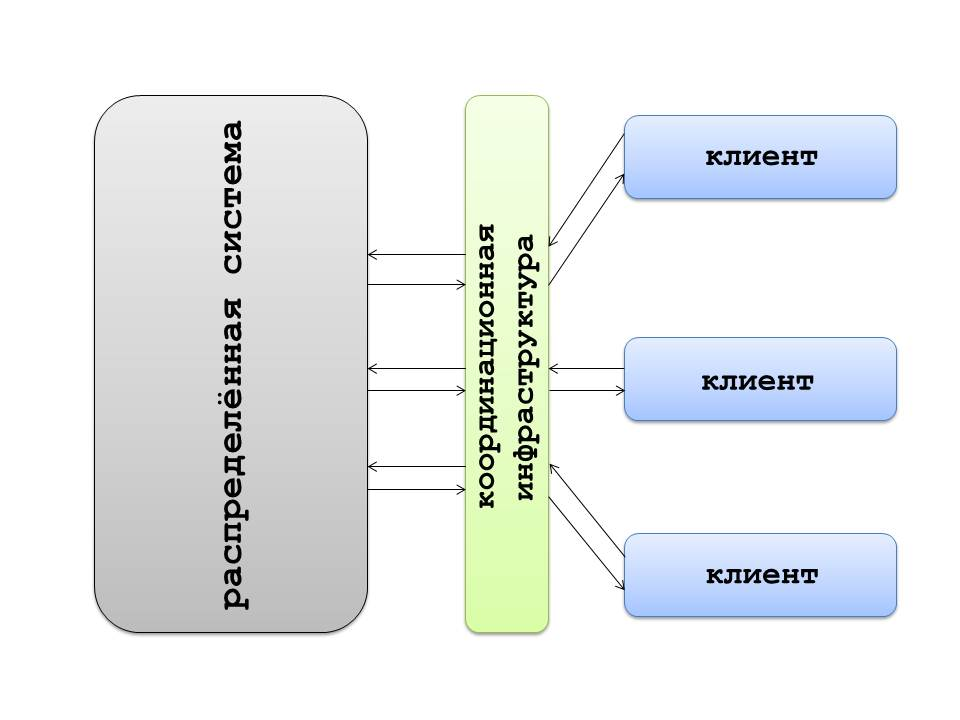
\includegraphics[width=0.7 \textwidth, height=0.5 \textwidth]{img/ClientServer}  \caption{Взаимодействие клиентов с~распределённой системой} \label{clser}
\end{figure}
Когда клиент~$p$ посылает запрос системе, этот запрос сначала обрабатывается координационной инфраструктурой и только после этого отправляется системе. При получении ответа от системы координационная инфраструктура также обрабатывает полученную информацию, а затем отправляет ответ клиенту~$p$. Поэтому клиентская часть операций чтения/записи исполняется на стороне координационной структуры, а не на стороне клиента.

Реализация системы \texttt{BTS} состоит из 4 модулей:
\begin{itemize}
	\item модуль \texttt{secondary\_functions} включает в себя вспомогательные функции,
	\item модуль \texttt{client} реализует клиентский интерфейс,
	\item модуль \texttt{BTS_infrastructure} реализует деятельность координационной инфраструктуры,
	\item модуль \texttt{BTS_server} реализует деятельность сервера $s \in U$.
\end{itemize}
Рассмотрим реализацию компонент более подробно.

\subsection{Модуль secondary_functions}\label{subsec:2}
Модуль \texttt{secondary\_functions} включает в себя функции сетевого взаимодействия (\texttt{get_message}, \texttt{send_message}, \texttt{connect_to_server}), а также функцию создания и записи пространства кортежей в файл (\texttt{create_ts_file}). Реализации данных функций представлены в листинге~\ref{list:secfunc} в приложении.

Функции сетевого взаимодействия используют в своей работе возможности модуля \texttt{socket} из стандартной бибилиотеки \texttt{Python}~\ref{socket}. Функция \texttt{connect_to_server} принимает в качестве входного параметра порт, к которому необходимо подключиться. При удачном подключении возвращается сокет, который можно использовать для обмена сообщениямив дальнейшей работе, иначе возвращается объект \texttt{None}, сигнализирующий о неудаче.

Функция \texttt{send_message} используются для отправки данных по сети, она имеет два входных параметра: сокет, с помощью которого осуществляется отправка сообщения, и само сообщение, которое требуется отправить. Чтобы преобразовать сообщение к виду, пригодному для записи в сокет, используется функция \texttt{dumps} из модуля \texttt{pickle}~\ref{pickle}, отвечающая за сериализацию объектов. После завершения операции записи в сокет функция \texttt{send_message} завершает свою работу.

Функция \texttt{get_message} используются для получения данных из сети, она имеет единственный входной параметр~--- сокет, из которого осуществляется чтение информации. Если полученное сообщение оказалось пустым, то возвращается объект \texttt{None}, иначе сообщение десериализуется с помощью функции \texttt{loads} из модуля \texttt{pickle} и возвращается функцией \texttt{get_message}.

Функция \texttt{create_ts_file} создаёт пространство кортежей и записывает его в файл. Данная функция используется для того, чтобы в дальнейшем каждый сервер системы при запуске смог прочитать информацию из созданного при помощи  \texttt{create_ts_file} файла и сконструировать локальную реплику пространства кортежей. Имя файла, объём создаваемого пространства, а также длина и значения полей входящих в него кортежей регулируются входными параметрами функции. Для преобразования созданного пространства кортежей в удобный формат и записи в файл используется функция \texttt{dump} из модуля \texttt{json}~\ref{json}.


\subsection{Модуль client}\label{subsec:3}
Интерфейс пользователя для взаимодействия с \texttt{BTS} реализован с помощью класса \texttt{Client} из модуля \texttt{client} (полный программный код представлен в приложении). Для того, чтобы начать работу, следует создать объект класса \texttt{Client}, передав конструктору в качестве входного параметра значение порта, который координационная инфраструктура использует для обмена сообщениями с клиентами.

Далее для исполнения операций чтения/записи нужно вызвать соответствующую функцию: \texttt{out_op($t$)}, \texttt{rd_op($\bar t$)} или \texttt{in_op($\bar t$)}. Заметим, что операция записи \texttt{out_op} в качестве входного параметра принимает кортеж, а операции чтения \texttt{rd_op} и \texttt{in_op} --- шаблон кортежа. Каждая из этих операций формирует запрос в виде словаря \texttt{\{'op': код операции, 'tup': кортеж\}} или \texttt{\{'op': код операции, 'temp': шаблон кортежа\}}, соответствующий её семантике. Сформированный запрос отправляется координационной инфраструктуре. Для завершения операции записи не требуется ответ системы, а операции чтения ожидают, когда инфраструктура вернёт запрошенное значение.

Для корректного завершения работы системы в классе \texttt{Client} реализована функция \texttt{stop_op()}, которая отправляет инфраструктуре запрос о прекращении работы и ожидает ответа об успешном результате операции. По смыслу данная функция не должна являться частью клиентского интерфейса, она была включена в класс \texttt{Client} для удобства.

Ввиду возможности возникновения ошибок для контроля исполнения операций используется модуль~\texttt{logging}~\ref{logging} из стандартной библиотеки языка \texttt{Python}, отвечающий за логирование. Создание и настройка конфигурации лога происходит в конструкторе класса \texttt{Client} при помощи функции \texttt{basicConfig}, устанавливающей имя файла для записи лога, формат выводимых сообщений и уровень логирования. Всего существует пять уровней логирования, в реализации использован уровень \texttt{INFO} для вывода информационных сообщений.

\subsection{Модуль BTS_infrastructure}\label{subsec:4}
Координационная инфраструктура системы \texttt{BTS} реализована в модуле \texttt{BTS_infrastructure} с помощью класса \texttt{BTS_infrastructure} (полный программный код представлен в приложении). Она представляет собой многопоточное приложение, которое обрабатывает запросы клиента и взаимодействует с серверами системы \texttt{BTS}.

Для того, чтобы настроить работу координационной системы, необходимо создать объект класса \texttt{BTS_infrastructure} и передать в его конструктор (см.\,листинг \ref{bts1}) следующие параметры:
\begin{itemize}
	\item порт, который будет прослушивать инфраструктура и на который будут поступать клиентские запросы,
	\item список портов, каждый из которых будет прослушивать определённый сервер системы \texttt{BTS},
	\item количество неисправных серверов (предателей), которые будут порождать конфликты в системе,
	\item размер кворума записи,
	\item размер кворума чтения,
	\item имя файла, в котором хранится множеством кортежей для корректных серверов,
	\item имя файла, в котором хранится множеством кортежей для неисправных серверов.
\end{itemize}
В теле конструктора значения входных параметров присваиваются соответствующим свойствам класса, устанавливается значение флага \texttt{THREAD_POOL_ON} (данный флаг используется при обработке клиентских запросов), значение свойства \texttt{AMOUNT_OF_CLIENTS} устанавливается в нуль (данное свойство является счётчиком поступивших клиентских запросов), множество серверов \texttt{self.U} разбивается на кворумы записи \texttt{Q_w} и чтения \texttt{Q_r}, а также настраивается конфигурация лога. 

После создания объекта класса для запуска работы координационной инфраструктуры необходимо вызвать метод \texttt{run} (см.\,листинг \ref{bts2}). Если изначально количество неисправных серверов было указано неверно, то есть не меньше количества всех имеющихся серверов, то возвращается значение \texttt{False}. Иначе работа функции продолжается: происходит запуск корректных и неисправных серверов с помощью метода \texttt{start_servers} (см.\,листинг \ref{bts1}).

Метод \texttt{start_servers} имеет три входных параметра:
\begin{itemize}
	\item два индекса, определяющих диапазон значений в списке портов \texttt{self.U}, которые будут прослушивать запускаемые серверы,
	\item имя файла, которое будет подано выбранным серверам на вход.
\end{itemize}
Программная реализация сервера системы \texttt{BTS} представлена в модуле \texttt{BTS_server}, который будет рассмотрен позже в разделе~\ref{subsec:5}, данный скрипт \texttt{BTS_server.py} запускается с определёнными параметрами в новом процессе при помощи конструктора класса \texttt{Popen} из модуля \texttt{subprocess} \ref{subprocess} стандартной библиотеки \texttt{Python}. В скрипт передаются следующие аргументы:
\begin{itemize}
	\item идентификатор сервера,
	\item порт, который будет прослушивать сервер,
	\item имя файла с хранящимся в нём пространством кортежей,
	\item список портов кворума, которому принадлежит сервер.
\end{itemize}
Информация об исполненных операциях записывается в лог инфраструктуры.

Вернёмся к методу \texttt{run}. После запуска серверов создаётся и настраивается сокет, с помощью которого далее будет происходить коммуникация с клиентскими процессами. Будем обрабатывать клиентские запросы при помощи пула потоков \texttt{ThreadPoolExecutor} из модуля \texttt{concurrent.futures} \ref{concurrent} стандартной библиотеки \texttt{Python}, принимающего в качестве аргумента количество потоков, используемых пулом потоков.

Пока флаг \texttt{THREAD_POOL_ON} равен \texttt{True}, исполняется следующая последовательность инструкций: ожидается подключение клиента к порту, создаётся соответствующий клиентский сокет, количество полученных клиентских запросов увеличивается на единицу. При удачном завершении описанных инструкций задача добавляется в очередь для исполнения пулом потоков с помощью метода \texttt{submit}, принимающего в качестве входных параметров имя функции (\texttt{worker}), которую необходимо исполнить в одном из потоков пула, и значения аргументов (клиентский сокет и \texttt{AMOUNT_OF_CLIENTS}), с которыми эта функция будет запущена.

Флаг \texttt{THREAD_POOL_ON} может изменить своё значение только при получении запроса о прекращении работы от клиента. Если это произошло, то новые задачи перестают добавляться в очередь пула потоков, ожидается завершение всех исполняющихся или ожидающих в очереди задач. После завершения работы пула потоков вызывается метод \texttt{stop_servers} (см.\,листинг \ref{bts1}), при исполнении которого всем запущенным серверам посылается запрос о прекращении работы. Информация о проделанных операциях записывается в лог инфраструктуры. На этом работа метода \texttt{run} завершается, возвращается значение \texttt{True}, свидетельствующее об успешном завершении работы координационной инфраструктуры.

Заметим, что метод \texttt{run} является блокирующим, то есть после запуска инфраструктуры продолжить дальнейшую работу до завершения работы инфраструктуры будет невозможно.

Рассмотрим метод \texttt{worker} (см.\,листинг \ref{bts2}) более подробно. Он выполняет функцию получения и обработки запроса клиента и принимает в качестве входных параметром клиентский сокет и идентификатор клиентского процесса. Вспомним, что в функцию \texttt{submit} (добавление задачи в очередь пула потоков) в качестве второго аргумента функции \texttt{worker} передаётся значение свойства \texttt{AMOUNT_OF_CLIENTS}. Данное свойство используется для подсчёта клиентских запросов, будем пологать, что каждый клиентский запрос был послан уникальным клиентом ( согласно системной модели \texttt{BTS} множество клиентских процессов бесконечно), тогда в качестве идентификатора клиентского процесса можно использовать номер запроса. Это осуществляется при помощи свойства \texttt{AMOUNT_OF_CLIENTS}.

Работу метода \texttt{self.worker} можно разделить на два этапа: получение сообщения от клиента и обработка полученного запроса. Для того, чтобы получить сообщение с запросом от клиента, используется функция \texttt{get_message} из описанного в разделе \ref{subsec:2} модуля \texttt{secondary\_functions}. После получения запроса определяется код операции, которую необходимо исполнить, вызывается соответствующая функция и при необходимости отправляется ответ клиенту.

При получении запросов на исполнение операций $out$, $rdp$ или $inp$ вызываются методы \texttt{out}, \texttt{rdp} или \texttt{inp}, которые будут рассмотрены позже в разделах \ref{}, \ref{} и \ref{} соответственно.

При получении запроса на исполнение операции $stop$ флаг \texttt{THREAD_POOL_ON} устанавливается в значение \texttt{False}, после чего прекращается обработка клиентских запросов, система готовится к завершению работы.


\subsection{Модуль BTS_server}\label{subsec:5}
Серверная часть системы \texttt{BTS} реализована в модуле \texttt{BTS_server} (полный программный код представлен в приложении), он представляет собой скрипт, запуск которого приводит в исполнение сервер системы. Как уже было отмечено в разделе \ref{subsec:4}, скрипт запускается со следующими аргументами:
\begin{itemize}
	\item идентификатор сервера,
	\item порт, который будет прослушивать сервер,
	\item имя файла с хранящимся в нём пространством кортежей,
	\item список портов кворума, которому принадлежит сервер.
\end{itemize}
Для обработки аргументов командной строки используется библиотека \texttt{argparse} \ref{argparse}. Она предоставляет возможности анализа аргументов командной строки, конвертирования стркоовых аргументов в другие объекты программы и вывода информационных подсказок.

Для мониторинга работы сервера настраивается логирование.

При запуске сервер считывает из полученного файла кортежи и создаёт локальную копию пространства кортежей при помощи функции \texttt{read_from_ts_file} (см.\,листинг \ref{server2}). На сервере кортежи хранятся в контейнере \texttt{set}, что позволяет исключить наличие идентичных кортежей и сделать проверку на вхождение быстрой, поскольку \texttt{set} в качестве базовой структуры данных использует хэш-таблицу \ref{Gorelick}.

Далее, как и в случае с координационной инфраструктурой, создаётся сокет, через который будет осуществляться коммуникация с инфраструктурой, запускается пул потоков \ref{threadpool} и начинается обработка входящих запросов.

Обработка входящих запросов осуществляется при помощи функции \texttt{worker}, программный код которой можно посмотреть в приложении в листинге \ref{server2}. В теле данной функции сначала происходит считывание сообщения, полученного от инфраструктуры, далее по содержимому полученного сообщения определяется тип комнады и вызывается соответствующая одноимённая функция. Полный перечень возможных команд приведён ниже:
\begin{itemize}
	\item \texttt{out} - команда операции записи $out$,
	\item \texttt{rd} - команда операции недеструктивного чтения $rd$,
	\item \texttt{in} - команда операции деструктивного чтения $in$,
	\item \texttt{enter} - команда входа в критическую секцию,
	\item \texttt{exit} - команда выхода из критической секции,
	\item \texttt{accept1} - команда первого этапа утверждения удаляемого кортежа,
	\item \texttt{accept2} - команда второго этапа утверждения удаляемого кортежа,
	\item \texttt{stop} - команда о прекращения работы сервера.
\end{itemize}
Первые три команды связаны с операциями манипулирования кортежами, следующие четыре команды связаны с реализацией операции $in$ и будут рассмотрены позже в разделах \ref{}. Последняя команда \texttt{stop} устанавливает флаг \texttt{THREAD_POOL_ON} в значение \texttt{False}, что приводит к прекращению работы пула потоков, а затем - к завершению работы сервера. Информация о произведённых действиях записывается в лог.


\subsection{Операция записи out}\label{subsec:6}
Операция~$out(t)$ добавляет кортеж $t$ в~пространство кортежей. На~стороне инфраструктуры эта операция реализуется с~помощью функции \texttt{out(self, t)}, программный код которой приведён в листинге \ref{} в приложении.

Для того, чтобы добавить кортеж $t$ в пространство, производится подключение к серверам системы, состоящим в кворуме записи, и в случае удачного подключения отправляется запрос \texttt{{'op': 'out', 'tup': t}} на добавление кортежа.

Заметим, что при~вызове данной функции ждать ответа от~серверов нет необходимости. Будем считать, что операция завершится в~тот момент, когда все корректные серверы из~кворума записи получат кортеж~$t$.

На~стороне сервера операция~$out(t)$ реализуется с~помощью функции \texttt{out(t)} (программный код приведён в листинге \ref{} в приложении). При~получении запроса на добавление кортеж~$t$ добавляется в~пространство кортежей только в~том случае, если этот кортеж ранее не~был из~него удалён (то есть его нет во множестве \texttt{RS}). Это необходимо для~того, чтобы один и тот же кортеж не~был удалён дважды.

\subsection{Операция чтения rd}\label{subsec:7}
Операция недеструктивного чтения~$rd(\bar t)$ в~качестве входного параментра принимает шаблон кортежа~$\bar t$ и возвращает копию соответствующего шаблону кортежа, не извлекая его из~пространства. На~стороне инфраструктуры эта операция реализуется с~помощью функции \texttt{rdp(self, temp, ts=None)}, имеющей два параметра: шаблон кортежа и объект \texttt{ts} по умолчанию равный \texttt{None}, значение которого будет объяснено позже. При получении запроса на исполнение операции $rd$ данная функция вызывается с единственным первым параметром. Программный код приведён в листинге \ref{} в приложении.

Суть работы функции заключается в следующем. Каждому серверу из кворума чтения посылается запрос на исполнение операции~$rd(\bar t)$. Ответы от серверов кворума приходят в виде множества подходящих под~шаблон~$\bar t$ кортежей и записываются в словарь \texttt{ts}, имеющий структуру: \texttt{port: (socket, set)}, где \texttt{port} - порт, который прослушивает конкретный сервер, \texttt{socket} - сокет, с помощью которого происходит коммуникация, \texttt{set} - множество подходящих кортежей, хранящихся на данном сервере. Заметим, что словарь \texttt{ts} может передаваться в функцию уже в готовом виде, этот факт используется в реализации операции~$in(\bar t)$, которая будет рассмотрена в разделе \ref{}.

Из всех полученных кортежей выбирается один общий кортеж~$t$, который располагается как минимум на~$f + 1$ сервере. Чтобы найти кортеж~$t$, необходимо подобрать такую комбинацию из~$f + 1$ сервера, пересечение множеств подходящих кортежей которых будет непусто. Для этого рассматриваются всевозможные сочетания из~$f + 1$ сервера при помощи функции \texttt{combinations} из модуля \texttt{itertools} \ref{itertools}. Для нахождения пересечений множеств подходящих кортежей используются методы класса \texttt{set} \ref{set}. После нахождения кортежа~$t$ он возвращается в качестве выходного параметра. Если подходящего кортежа не нашлось, то возвращается объект \texttt{None}, свидетельствующий о том, что операция чтения не~увенчалась успехом.

Рассмотрим реализацию операции недеструктивного чтения на стороне сервера с помощью функции \texttt{rdp(sock, temp)}, принимающей два входных параметра: сокет для обмена сообщениями и шаблон кортежа (программный код представлен в листинге \ref{} в приложении). Для того, чтобы найти подходящие под шаблон кортежи, производится один проход по локальной копии пространства кортежей \texttt{TS}, каждый кортеж которого проверяется на пригодность функцией \texttt{match}. Если функция \texttt{match} вернула значение \texttt{True}, то кортеж добавляется во множество подходящих кортежей \texttt{temp_set}.

Функция \texttt{match(temp, t)} сравнивает длины шаблона и кортежа, в случае совпадения длин сравниваются определённые в шаблоне поля с соответствующими полями проверяемого кортежа. Если длины кортежей оказались разными или какое-то определённое поле шаблона не совпало с соответствующим полем кортежа, то возвращается значение \texttt{False}, говорящее о том, что кортеж не подходит под шаблон. Иначе возвращается значение \texttt{True}.

Если переданный в функцию \texttt{rdp} сокет оказался не равен значению \texttt{None}, то полученное множество \texttt{temp_set} отправляется инфрструктуре в качестве ответа. Иначе оно возвращается в качестве выходного параметра. Такая архитектура необходима для реализации операции~$in(\bar t)$, которая будет рассмотрена в разделе \ref{}.




\subsection{Операция чтения inp}\label{subsec:8}
Операция~$inp$ является операцией деструктивного чтения, она имеет более сложную реализацию, поскольку один кортеж не~может быть удалён из~пространства двумя различными вызовами~$inp$. Этот факт подразумевает использование критических секций для~процессов, пытающихся удалить один и тот же кортеж, что, во-первых, обеспечит невозможность удаления кортежа двумя процессами одновременно, во-вторых, позволит всем процессам получить доступ к~ресурсу в~некоторое время. Операции входа в критическую секцию на~стороне клиента реализуется с~помощью функции~$enter(\bar t)$, описанной в~алгоритме\,\ref{alg5}:

\begin{algorithm}[H]
	\caption{Операция enter}\label{alg5}
	\begin{algorithmic}[1]
		\Statex $\{$client $p \}$
		\Function{enter}{$\bar t$}
		\State $T[s_1, \dots, s_{|Q_r|}] \gets (\perp, \dots, \perp)$
		
		\ForAll {$s \in U$}
		\State \Call{send}{$s, \langle$ ENTER, $p, \bar t \rangle$}
		\State $T[s] \gets T_s^{\bar t}$
		\EndFor
		
		\ForAll {$s \in Q_r$}
		\State \Wait{receive}{$s, \langle$ GO, $p, T_s^{\bar t} \rangle$}
		\State $T[s] \gets T_s^{\bar t}$
		\EndFor
		
		\If{$\exists t$ : ($|s$ : $t \in T[s]| \geqslant f + 1$)}
		\State \Return{$t$}
		\EndIf
		\State \Return{$\perp$}
		\EndFunction
	\end{algorithmic}
\end{algorithm}

Операция~$enter(\bar t)$ имеет входной параметр~--- шаблон кортежа, который требуется удалить в~результате исполнения операции~$inp$. Входной параметр нужен для~того, чтобы совместить операции входа в~критическую секцию и операцию чтения~$rdp$, что позволит уменьшить количество этапов коммуникации на~единицу. Сначала клиент~$p$ отправляет всем серверам запрос на~разрешение войти в~критическую секцию, затем ожидает, когда все серверы из~кворума чтения дадут положительный ответ на~отправленный запрос. При~отправке разрешения войти в~критическую секцию сервер~$s$ также отправляет список подходящих для~удаления кортежей (то~есть соответствующих шаблону~$\bar t$). Далее, как и в~реализации операции~$rdp$, из~всевозможных вариантов, присланных серверами, выбирается и возвращается общий кортеж~$t$, располагающийся хотя бы на~$f + 1$ сервере, иначе возвращается спецсимвол~$\perp$.

Операция выхода из~критической секции~$exit(\bar t)$ на~стороне клиента имеет более простую структуру: клиент~$p$ отсылает всем серверам сообщение о~выходе из~критической секции, не~дожидаясь какого-либо ответа от~них. Реализация данной операции представлена в~алгоритме\,\ref{alg6}:

\begin{algorithm}[H]
	\caption{Операция exit}\label{alg6}
	\begin{algorithmic}[1]
		\Statex $\{$client $p \}$
		\Procedure{exit}{$\bar t$}
		\ForAll {$s \in U$}
		\State \Wait{send}{$s, \langle$ EXIT, $p, \bar t \rangle$}
		\EndFor
		\EndProcedure
	\end{algorithmic}
\end{algorithm}

Рассмотрим операции входа в~критическую секцию и выхода из~неё на~стороне сервера. /здесь будет псевдокод и описание соответствующих алгоритмов/

Теперь рассмотрим реализацию операции~$inp$ (см.\,алгоритм\,\ref{alg9}). В~первую очередь клиент~$p$ пытается войти в~критическую секцию для~удаления подходящего под~шаблон~$\bar t$ кортежа. По~окончании выполнения функции~$enter(\bar t)$ все серверы из~кворума чтения уже разрешили войти в~критическую секцию, а клиент~$p$ уже выбрал конкретный кортеж~$t$ для~удаления.

\begin{algorithm}[H]
	\caption{Операция inp}\label{alg9}
	\begin{algorithmic}[1]
		\Statex $\{$client $p \}$
		\Function{inp}{$\bar t$}
		\Repeat
			\State $t \gets$ \Call{enter}{$\bar t$}
			\If{$t = \perp$}
				\State \Call{exit}{$\bar t$}
				\State \Return{$\perp$}
			\EndIf
			\State $d \gets$ \Call{paxos}{$p, P, A, L, t$}
			\State \Call{exit}{$\bar t$}
		\Until{$d = t$}
		\State \Return{$t$}
		\EndFunction
	\end{algorithmic}
\end{algorithm}

Если выбранный кортеж~$t$ оказался равен спецсимволу~$\perp$, значит в~пространстве кортежей нет ни~одного подходящего под~шаблон~$\bar t$ кортежа, в~этом случае клиент~$p$ выходит из~критической секции, а в~качестве результата возвращается спецсимвол~$\perp$, сигнализирующий о~неудачном завершении операции~$inp$.

Если выбранный кортеж~$t$ не~равен спецсимволу~$\perp$, то клиент~$p$ предлагает серверам удалить именно его. Для~того, чтобы удалить кортеж~$t$, соответствующий шаблону~$\bar{t}$, из~пространства, серверы из~кворума чтения должны принять решение, можно~ли удалить кортеж~$t$. Для~этой цели вызывается функция~$paxos$, являющаяся реализацией алгоритма достижения консенсуса в~распределённых системах. Данная функция имеет пять параметров: 
\begin{enumerate}
	\item Процесс~$p$, предлагающий значение. В~нашем случае это клиентский процесс, вошедший в~критическую секцию.
	\item Множество Заявителей~$P = \{p, s_1, ..., s_{f+1}\}$, состоящее из~клиентского процесса~$p$ и $f + 1$~сервера. Такой набор гарантирует наличие хотя~бы одного корректного заявителя.
	\item Множество Акцепторов~$A = U$. Все серверы являются Акцепторами.
	\item Множество Узнающих~$L = \{p\} \cup U$. О~принятом решении узнают все серверы и клиентский процесс.
	\item Предлагаемое значение~$t$.
\end{enumerate}

В~качестве выходного параметра~$paxos$ возвращает кортеж~$d$, который было принято удалить из~пространства. Далее происходит выход из~критической секции. Если полученное значение~$d$ совпало с~предлагаемым~$t$, то операция~$inp$ завершается и возвращает в~качестве выходного параметра удалённый кортеж~$t$. Если~$d \ne t$, то все вышеописанные выкладки проделываются заново до~тех~пор, пока не~выполнится условие~$d = t$.

На~момент выхода из~функции~$paxos$ все Акцепторы уже приняли решение, удалять кортеж~$t$ или нет, все Узнающие получили сообщения о~решении Акцепторов. Если функция~$paxos$ вернула кортеж, то он уже был удалён из~пространства кортежей, иначе возвращается спецсимвол~$\perp$, сигнализирующий о~том, что операция удаления кортежа~$t$ не~увенчалась успехом. Данный результат иллюстрирует благоприятный и промежуточный исходы задачи византийских генералов. При~благоприятном исходе из~пространства кортежей удаляется кортеж, предложенный клиентом, то~есть приказ главнокомандующего (клиента) был получен и изучен всеми генералами (серверами), после~чего они единогласно приняли решение следовать приказу. При~промежуточном исходе кортеж не~удаляется, возвращается спецсимвол~$\perp$, при~этом сохраняется целостность пространства кортежей, поскольку на~всех корректных серверах удаления не~произошло. Иными словами, генералами (серверами) было принято единогласное решение не~доверять приказу главнокомандующего (клиента) и отступить (не~производить удаление), сохранив при~этом армию (целостность пространства кортежей).

/здесь будет описание серверной части операции inp/

\subsection{Блокирующие операция rd и in}\label{subsec5:4}
Кроме того, операции чтения являются блокирующими, то~есть если в~пространстве кортежей на данный момент нет ни~одного кортежа, соответствующего шаблону, то процесс, пославший запрос, заблокируется до~того момента, пока в~пространстве не~появится подходящего кортежа.

Блокирующие операции $rd$ и $in$, соответствующие спецификации языка~$Linda$, могут быть реализованы на~стороне клиента путём повторного вызова их неблокирующих аналогов $rdp$ и $inp$ до~тех~пор, пока необходимый кортеж не~будет получен.





\Conc

\printbibliography[heading=bibintoc]

\appendix
\ifthenelse{\value{worktype} > 1}{%
	\addtocontents{toc}{%
		\protect\renewcommand{\protect\cftchappresnum}{\appendixname\space}%
		\protect\addtolength{\protect\cftchapnumwidth}{\widthof{\appendixname\space{}} - \widthof{Глава }}%
	}%
}{
\addtocontents{toc}{%
	\protect\renewcommand{\protect\cftsecpresnum}{\appendixname\space}%
	\protect\addtolength{\protect\cftsecnumwidth}{\widthof{\appendixname\space{}}}%
}%
}
\section*{Приложение}
\addcontentsline{toc}{section}{Приложение}
\begin{ListingEnv}[H]\caption{Модуль \texttt{secondary\_functions}}\label{list:secfunc}
\begin{lstlisting}[language=Python, numbers=left]
from socket import socket, AF_INET, SOCK_STREAM, error
import pickle
import json

def get_message(sock):
  sock.settimeout(50)
  msg = b""
  tmp = b""
  while True:
	try:
	  tmp = sock.recv(1024)
	except error:
	  break
	if len(tmp) < 1024:
	  break
	msg += tmp
  msg += tmp
  if len(msg) > 0:
	return pickle.loads(msg)
  else:
	return  None

def send_message(sock, msg):
  sock.send(pickle.dumps(msg))

def connect_to_server(port):
  sock = socket(AF_INET, SOCK_STREAM)
  i = 50
  while i:
	try:
	  sock.connect(('localhost', port))
	except ConnectionRefusedError:
	  i -= 1
	else:
	  return sock
  return None

def create_ts_file(file_name, init_num, amount=500, length=100):
  with open(file_name, 'w') as f:
	list_of_tuples = list()
	for i in range(init_num * amount, (init_num + 1) * amount):
	  list_of_tuples.append(tuple(j for j in range(i, i + length)))
	json.dump(list_of_tuples, f)
	
	\end{lstlisting}
\end{ListingEnv}

\begin{ListingEnv}[p]\caption{Класс \texttt{Client}, модуль \texttt{client}}\label{list:client}
\begin{lstlisting}[language=Python, numbers=left]
import logging
from secondary_functions import get_message, send_message, connect_to_server

class Client(object):

  def __init__(self, port):
	self.port = port
	logging.basicConfig(filename='client_log.txt', level=logging.DEBUG, format="%(asctime)s - %(message)s")


  def out_op(self, tup):
	sock = connect_to_server(self.port)

	if sock is not None:
	  send_message(sock, {'op': 'out', 'tup': tup})
	  sock.close()
	  logging.info('OUT: ' + str(tup))
	else:
	  logging.info('OUT_OP: cannot connect to server')

	
  def rd_op(self, temp):
	sock = connect_to_server(self.port)

	if sock is not None:
	  send_message(sock, {'op': 'rdp', 'temp': temp})
	  resp = get_message(sock)
	  sock.close()
	  logging.info('RD: ' + str(resp['resp']))

	  if resp is None:
		return resp
	  else:
		return resp['resp']
	else:
	  logging.info('RD_OP: cannot connect to server')
	  return None

\end{lstlisting}
\end{ListingEnv}
\begin{ListingEnv}[p]\caption{Класс \texttt{Client}, модуль \texttt{client} (продолжение)}\label{list:client2}
\begin{lstlisting}[language=Python, numbers=left]
  def in_op(self, temp):
  
	sock = connect_to_server(self.port)

	if sock is not None:
	  send_message(sock, {'op': 'inp', 'temp': temp})
	  resp = get_message(sock)
	  sock.close()
	  logging.info('In: ' + str(resp['resp']))

	  if resp is None:
		return resp
	  else:
		ret	urn resp['resp']

	else:
	  logging.info('IN_OP: cannot connect to server')
	  
	  return None
	
  def stop_op(self):
  
	sock = connect_to_server(self.port)

	if sock is not None:
	  send_message(sock, {'op': 'stop'})
	  resp = get_message(sock)
	  sock.close()
	  logging.info('STOP_OP: ' + str(resp['resp']))

	  if resp is None:
		return resp
	  else:
		return resp['resp']

	else:
	  logging.info('STOP_OP: cannot connect to server')
	  
	  return None
	
	\end{lstlisting}
\end{ListingEnv}

\begin{ListingEnv}[p]\caption{Класс~\texttt{\small BTS_infrastructure}, модуль~\texttt{\small BTS_infrastructure}}\label{list:bts1}
\begin{lstlisting}[language=Python, numbers=left]
from secondary_functions import *
from subprocess import Popen, CalledProcessError, PIPE
from concurrent.futures import ThreadPoolExecutor
from itertools import combinations
from collections import Counter
import logging

class BTS_infrastructure(object):
  def __init__(self, port, servers, amount_of_enemies, size_of_QW, size_of_QR, right_file, wrong_file):
    self.INFRASTRUCTURE_PORT = port
    self.U = servers
    self.AMOUNT_OF_SERVERS = len(servers)
    self.AMOUNT_OF_ENEMIES = amount_of_enemies
    self.TS_FILE, self.WRONG_TS_FILE = right_file, wrong_file
    self.THREAD_POOL_ON = True
    self.AMOUNT_OF_CLIENTS = 0
    self.QW, self.QR = self.U[0:size_of_QW], self.U[-size_of_QR:]
    logging.basicConfig(filename='infrastructure_log.txt', level=logging.DEBUG, format="%(asctime)s - %(message)s")
    logging.info('Infrastructure on port ' + str(self.INFRASTRUCTURE_PORT))

  def start_servers(self, ind1, ind2, file):
    for i in range(ind1, ind2):
      if U[i] in self.QR:
        quorum = self.QR
      else:
        quorum = [U[i]]

    try:
      Popen('python BTS_server.py '+str(i)+' '+str(self.U[i])+' '+str(file)+' '+''.join(str(j)+' ' for j in quorum), stdout=PIPE, stderr=PIPE, shell=True)
    except CalledProcessError:
      logging.info("START_SERVERS: cannot start server "+str(self.U[i]))
    else:
      logging.info("START_SERVERS: start server "+str(self.U[i]))

  def stop_servers(self):
    for i in self.U:
      s = connect_to_server(i)
      if s is not None:
        send_message(s, {'op': 'stop'})
        s.close()
        logging.info("STOP_SERVERS: stop server "+str(i))
      else:
        logging.info("STOP_SERVERS: cannot stop server "+str(i))
        
\end{lstlisting}
\end{ListingEnv}
\begin{ListingEnv}[p]\caption{Класс~\texttt{\small BTS_infrastructure}, модуль~\texttt{\small BTS_infrastructure} (продолжение)}\label{list:bts2}
	\begin{lstlisting}[language=Python, numbers=left]        
  def worker(self, client, pid):
    req = get_message(client)
    try:
      if req['op'] == 'out':
        self.out(req['tup'])
      elif req['op'] == 'rdp':
        send_message(client, {'resp':self.rdp(req['temp'])})
      elif req['op'] == 'inp':
        send_message(client, {'resp':self.inp(pid,req['temp'])})
      elif req['op'] == 'stop':
        self.THREAD_POOL_ON = False
        send_message(client, {'resp': 'ok'})
      else:
        logging.info('WORKER: wrong request ' + str(req))
    except KeyError:
      logging.info('WORKER: wrong request ' + str(req))
    client.close()
  
  def run(self):
    if self.AMOUNT_OF_ENEMIES >= self.AMOUNT_OF_SERVERS:
      return False
      
    self.start_servers(0,self.AMOUNT_OF_ENEMIES,self.WRONG_TS_FILE)
    self.start_servers(self.AMOUNT_OF_ENEMIES,self.AMOUNT_OF_SERVERS,self.TS_FILE)
    
    s = socket(AF_INET, SOCK_STREAM)
    s.bind(('', self.INFRASTRUCTURE_PORT))
    s.listen(1)
  
    with ThreadPoolExecutor(4) as pool:
      while self.THREAD_POOL_ON:
        try:
          s.settimeout(30)
          client_s, client_addr = s.accept()
          self.AMOUNT_OF_CLIENTS += 1
        except error:
          pass
        else:
          pool.submit(self.worker, client_s, self.AMOUNT_OF_CLIENTS)
  
    self.stop_servers()
    s.close()
    logging.info('RUN: stop working')
    return True
    
	\end{lstlisting}
\end{ListingEnv}
\begin{ListingEnv}[p]\caption{Класс~\texttt{\small BTS_infrastructure}, модуль~\texttt{\small BTS_infrastructure} (продолжение)}\label{list:bts3}
	\begin{lstlisting}[language=Python, numbers=left]        
  def enter_r(self, pid, temp):
    ts = {i: [None, None] for i in self.U}  # port: (socket, set)
    
    for i in self.U:
      ts[i][0] = connect_to_server(i)
      if ts[i][0] is not None:
        send_message(ts[i][0], {'op': 'enter', 'pid': pid, 'temp': temp})
        logging.info('ENTER_R: send ' + str(temp) + ' to server ' + str(i))
      else:
        if i in self.QR:
          return tuple([None, None])
        else:
          ts.pop(i)

    qr = set()
    
    for i in ts.keys():
      resp = get_message(ts[i][0])
      ts[i][0].close()
      
      if resp is None or resp['resp'] != 'go':
        logging.info('ENTER_R: wrong respond from server ' + str(i))
        ts[i][1] = None
      else:
        ts[i][1] = resp['ts']
        qr.add(i)
        
    if not set(self.QR).issubset(qr):
      return tuple([None, None])

    return tuple([self.rdp(temp, ts), ts])



  def exit_r(self, pid):
    for i in self.U:
      sock = connect_to_server(i)
      
      if sock is not None:
        send_message(sock, {'op': 'exit', 'pid': pid})
        sock.close()
      else:
        logging.info('EXIT_R: cannot exit cs with pid: ' + str(pid))
    
	\end{lstlisting}
\end{ListingEnv}
\begin{ListingEnv}[p]\caption{Класс~\texttt{\small BTS_infrastructure}, модуль~\texttt{\small BTS_infrastructure} (продолжение)}\label{list:bts4}
	\begin{lstlisting}[language=Python, numbers=left]        
  def out(self, t):
  for i in self.QW:
    sock = connect_to_server(i)
    if sock is not None:
      send_message(sock, {'op': 'out', 'tup': t})
      logging.info('OUT: send ' + str(t) + ' to server ' + str(i))
      sock.close()
    else:
      logging.info('OUT: cannot connect to server ' + str(i))


  def inp(self, pid, temp):
  while True:
    t, ts = self.enter_r(pid, temp)
    logging.info('INP: enter with pid ' + str(pid) + ', temp ' + str(temp) + ', t: ' + str(t))
    if t is None:
      self.exit_r(pid)
      logging.info('INP: exit from cs with pid ' + str(pid))
      return None

    d = self.paxos(pid, t, ts)
    self.exit_r(pid)
    logging.info('INP: exit from cs with pid ' + str(pid))
    if d == t:
      break

    return t


  def paxos(self, pid, t, ts):
    for i in ts.keys():
    ts[i][0] = connect_to_server(i)
    if ts[i][0] is not None:
      send_message(ts[i][0], {'op': 'in', 'pid': pid, 'tup': t})
    
    tup_list = []
    for i in ts.keys():
      resp = get_message(ts[i][0])
      ts[i][0].close()
      if resp is not None:
        tup_list.append(resp['resp'])
      else:
        tup_list.append(None)
    
    c = Counter(tup_list)
    return c.most_common(1)[0][0]
    
	\end{lstlisting}
\end{ListingEnv}
\begin{ListingEnv}[p]\caption{Класс~\texttt{\small BTS_infrastructure}, модуль~\texttt{\small BTS_infrastructure} (продолжение)}\label{list:bts5}
	\begin{lstlisting}[language=Python, numbers=left]        
  def rdp(self, temp, ts=None):
    if ts is None:
      ts = {i: [None, None] for i in self.U}  # port: (socket, set)
      for i in self.U:
        ts[i][0] = connect_to_server(i)
        if ts[i][0] is not None:
          send_message(ts[i][0], {'op': 'rd', 'temp': temp})
          logging.info('RDP:send '+str(temp)+'to server '+str(i))
        else:
          ts.pop(i)
  
      qr = set()
      for i in ts.keys():
        msg = get_message(ts[i][0])
        ts[i][0].close()
        if msg is not None:
          ts[i][1] = msg['ts']
          qr.add(i)
        else:
          ts[i][1] = None
          
        logging.info('RDP: receive ' + str(ts[i][1]) + ' from server ' + str(i))
        if not set(self.QR).issubset(qr):
          return None
  
    t = None
    for i in combinations(ts.keys(), self.AMOUNT_OF_ENEMIES + 1):
      ts_intersection = ts[i[0]][1]
 
      for j in i:
        if ts[j][1] is None:
          ts_intersection = None
          break
          
        ts_intersection = ts_intersection.intersection(ts[j][1])
        if len(ts_intersection) == 0:
          break
  
      if ts_intersection is None:
        continue
  
      if len(ts_intersection) > 0:
        t = ts_intersection.pop()
        break
  
    return t
	
	\end{lstlisting}
\end{ListingEnv}



\begin{ListingEnv}[p]\caption{Модуль~\texttt{BTS_server}}\label{list:server1}
	\begin{lstlisting}[language=Python, numbers=left]
from secondary_functions import *
import argparse
from concurrent.futures import ThreadPoolExecutor
from collections import deque
from collections import Counter
import logging

TS = set()
RS = set()
QR = deque()

SERVER_ID = 0
SERVER_PORT = 0
SERVERS = []

DECISIONS1 = {}
AMOUNT_OF_DECISIONS1 = 0

DECISIONS2 = {}
AMOUNT_OF_DECISIONS2 = 0

THREAD_POOL_ON = True
IS_ACCEPTED1 = False
IS_ACCEPTED2 = False



def read_from_ts_file(file_name):
  global TS
  
  with open(file_name, 'r') as f:
    data = json.load(f)
    for i in data:
      TS.add(tuple(i))
      
      
def match(temp, tup):
  if len(temp) != len(tup):
    return False

  for i, j in zip(temp, tup):
    if i is None:
      continue
    elif i != j:
      return False

  return True
	\end{lstlisting}
\end{ListingEnv}
\begin{ListingEnv}[p]\caption{Модуль~\texttt{BTS_server} (продолжение)}\label{list:server2}
	\begin{lstlisting}[language=Python, numbers=left]
def worker(client):
  global THREAD_POOL_ON
  
  req = get_message(client)

  if req['op'] == 'out':
    out(req['tup'])
  elif req['op'] == 'rd':
    rdp(client, req['temp'])
  elif req['op'] == 'in':
    inp(client, req['pid'], req['tup'])
    
  elif req['op'] == 'enter':
    enter_r(client, req['pid'], req['temp'])
  elif req['op'] == 'exit':
    exit_r(req['pid'])
    
  elif req['op'] == 'accept1':
    accept1(req['pid'], req['port'], req['tup'])
  elif req['op'] == 'accept2':
    accept2(req['pid'], req['port'], req['tup_dict'])
    
  elif req['op'] == 'stop':
    logging.info('WORKER: stop-message received')
    THREAD_POOL_ON = False
  
  else:
    logging.info('WORKER: wrong request ' + str(req))

  client.close()


def out(t):
  global TS, RS
  
  if t not in RS:
    TS.add(t)
    logging.info('OUT: add ' + str(t) + ' to TS')

  try:
    RS.remove(t)
  except KeyError:
    pass
  else:
    logging.info('OUT: remove ' + str(t) + ' from RS')

	\end{lstlisting}
\end{ListingEnv}
\begin{ListingEnv}[p]\caption{Модуль~\texttt{BTS_server} (продолжение)}\label{list:server3}
	\begin{lstlisting}[language=Python, numbers=left]  
def rdp(sock, temp):
  global TS
  temp_set = set()

  for t in TS:
    if match(temp, t):
      temp_set.add(t)

  logging.info('RDP: temp_set for ' + str(temp) + ' : ' + str(temp_set))
  if sock is not None:
    send_message(sock, {'ts': temp_set})
  else:
    return temp_set
  
def inp(sock, pid, tup):
  global TS, RS, QR
  if QR[0][1] == pid:
    d = paxos(sock, tup)
    if d is not None:
      if d not in TS:
        RS.add(d)
        logging.info('INP ' + str(pid) + ': add ' + str(d) + ' to RS')
      TS.remove(d)

def enter_r(sock, pid, temp):
  global QR
  QR.append((sock, pid, temp))
  if QR[0][1] == pid:
    logging.info('ENTER_R: ' + str(pid) + ' enter cs')
    temp_set = rdp(None, temp)
    send_message(sock, {'resp': 'go', 'ts': temp_set})

	\end{lstlisting}
\end{ListingEnv}
\begin{ListingEnv}[p]\caption{Модуль~\texttt{BTS_server} (продолжение)}\label{list:server4}
\begin{lstlisting}[language=Python, numbers=left]
parser = argparse.ArgumentParser()
parser.add_argument('id', type=int)
parser.add_argument('port', type=int)
parser.add_argument('TSFile', type=str)
parser.add_argument('quorum', nargs='+', type=int)
args = parser.parse_args()
SERVER_ID, SERVER_PORT, ts_file, SERVERS = args.id, args.port, args.TSFile, args.quorum

logging.basicConfig(filename=str(SERVER_ID) + 'log.txt', level=logging.DEBUG, format="%(asctime)s - %(message)s")
logging.info('Server ' + str(SERVER_ID) + ' on port ' + str(SERVER_PORT))
read_from_ts_file(ts_file)
logging.info('Read from file: ' + str(ts_file))
s = socket(AF_INET, SOCK_STREAM)
s.bind(('', SERVER_PORT))
s.listen(1)

with ThreadPoolExecutor(10) as pool:
  while THREAD_POOL_ON:
    try:
      s.settimeout(30)
      client_s, client_addr = s.accept()
    except error:
      pass
    else:
      pool.submit(worker, client_s)

s.close()
logging.info('RUN: stop working')
	\end{lstlisting}
\end{ListingEnv}



\if 0
Клиент~$p$ взаимодействует с~кворумом серверов чтения, в~качестве ответа на~запрос он получает от~каждого сервера список подходящих под~шаблон кортежей (серверная часть реализуется с~помощью алгоритма\,\ref{alg4}), затем клиент $p$ выбирает из~них общий кортеж~$t$, который располагается как минимум на~$f + 1$ сервере. Если такого кортежа нет, то возвращается спецсимвол~$\perp$, обозначающий, что операция не~увенчалась успехом. Заметим, что операция~$rdp$ не~является блокирующей в~отличие от~её аналога~$rd$ в~языке~$Linda$.

\begin{algorithm}[H]
	\caption{Операция out}\label{alg1}
	\begin{algorithmic}[1]
		\Statex $\{$client $p \}$
		\Procedure{out}{$t$}
		\ForAll {$s \in Q_w$}
		\State \Call{send}{$s, \langle$ OUT, $t \rangle$}
		\EndFor
		\EndProcedure
	\end{algorithmic}
\end{algorithm}

\begin{algorithm}[H]
	\caption{Операция out}\label{alg2}
	\begin{algorithmic}[1]
		\Statex $\{$server $s \}$
		\Upon{receive}{$p, \langle$ OUT, $t \rangle$}
		\If{$t \notin R_s$}
		\State $T_s \gets T_s \cup \{t\}$
		\EndIf
		\State $R_s \gets R_s \setminus \{t\}$
		\EndUpon
	\end{algorithmic}
\end{algorithm}

\begin{algorithm}[H]
	\caption{Операция rdp}\label{alg3}
	\begin{algorithmic}[1]
		\Statex $\{$client $p \}$
		\Function{rdp}{$\bar t$}
		\State $T[s_1, \dots, s_n] \gets (\perp, \dots, \perp)$
		
		\ForAll {$s \in U$}
		\State \Call{send}{$s, \langle$ RD, $\bar t \rangle$}
		\EndFor
		
		\Repeat
		\State \Wait{receive}{$s, \langle$ TS, $T_s^{\bar t} \rangle$}
		\State $T[s] \gets T_s^{\bar t}$
		\Until{$\{s \in U$ : $T[s] \ne \perp \} \in \mathcal{Q}_r$}
		
		\If{$\exists t$ : ($|s$ : $t \in T[s]| \geqslant f + 1$)}
		\State \Return{$t$}
		\EndIf
		\State \Return{$\perp$}
		\EndFunction
	\end{algorithmic}
\end{algorithm}

\begin{algorithm}[H]
	\caption{Операция rdp}\label{alg4}
	\begin{algorithmic}[1]
		\Statex $\{$server $s \}$
		\Upon{receive}{$p, \langle$ RD, $t \rangle$}
		\State $T_s^{\bar t} \gets \{t \in T_s$ : $m(t, \bar t)\}$
		\State send(p, $\langle$ TS, $T_s^{\bar t}\rangle$)
		\EndUpon
	\end{algorithmic}
\end{algorithm}


\fi

\if 0
% Если typeOfWork в SETUP.tex задан как 2 или 3, то начинать
% надо не с section (раздел), а с главы (chapter)
\section{Несколько примеров в~\LaTeX{}}
\label{sec:examples}
\subsection{Как вставлять листинги и рисунки}
Для крупных листингов есть два способа. Первый красивый, но в нём не допускается
кириллица (у вас может встречаться в комментариях и
печатаемых сообщениях), он представлен на листинге~\ref{list:hwbeauty}.
\begin{ListingEnv}[H]% буква H означает Here, t (top, сверху страницы),
% или b (bottom) или p (page, на отдельной странице)
\begin{lstlisting}
#include <iostream>
using namespace std;

int main()
{
    cout << "Hello, world" << endl;
    system("pause");
    return 0;
}
\end{lstlisting}
\caption{Программа “Hello, world” на \protect\cpp}\label{list:hwbeauty}
\end{ListingEnv}

Второй не такой красивый, но без ограничений (см.~листинг~\ref{list:hwplain}).
\begin{ListingEnv}[H]
\begin{Verb}

#include <iostream>
using namespace std;

int main()
{
    cout << "Привет, мир" << endl;
}
\end{Verb}
\caption{Программа “Hello, world” без подсветки}
\label{list:hwplain}
\end{ListingEnv}
 Приведём такой пример с указанием языка программирования, отличного от заданного по умолчанию:
\begin{lstlisting}[language=Haskell]
fibs = 0 : 1 : zipWith (+) fibs (tail fibs)
\end{lstlisting}
Такое решение~--- со вставкой нумерованных листингов покрупнее
и вставок без выделения для маленьких фрагментов~--- выбрано,
например, в книге Эндрю Таненбаума и Тодда Остина по архитектуре
компьютера~\autocite{TanAus2013} (см.~рис.~\ref{fig:tan-aus}).

Наконец, для оформления идентификаторов внутри строк
(функция \lstinline{main} и тому подобное) используется
\texttt{lstinline} или, самое простое, моноширинный текст
(\texttt{\textbackslash texttt}).

\subsection{Как оформить таблицу}

Для таблиц обычно используются окружения table и tabular --- см. таблицу~\ref{tab:widgets}. Внутри окружения tabular используются специальные команды пакета booktabs — они очень красивые; самое главное: использование вертикальных линеек считается моветоном.

\begin{table}
\centering
\caption{\label{tab:widgets}Подпись к таблице --- сверху}
\begin{tabular}{llr}
\toprule
\multicolumn{2}{c}{Item} \\
\cmidrule(r){1-2}
Животное  & Описание    & Цена (\$) \\
\midrule
Gnat      & per gram    & 13.65      \\
          & each        & 0.01       \\
Gnu       & stuffed     & 92.50      \\
Emu       & stuffed     & 33.33      \\
Armadillo & frozen      & 8.99       \\
\bottomrule
\end{tabular}
\end{table}

\fi

\end{document}
